\documentclass[12pt]{article}
\usepackage{amsmath, amssymb, geometry, graphicx, times}
\usepackage{mathptmx}  
\usepackage{fontspec}
\usepackage{xeCJK} % 处理中文
\usepackage{unicode-math} % 处理数学字体
\usepackage{listings}
% 设置英文字体(Times New Roman)
\setmainfont{Times New Roman}

% 设置数学字体(可以使用 Times New Roman 或其他更好的数学字体)
\setmathfont{TeX Gyre Termes Math}

% 设置中文字体(宋体)
\setCJKmainfont{SimSun} % Windows系统的宋体
\geometry{a4paper, margin=1in}

\title{有限元编程作业}
\author{Name: Yixuan Jiang \\ Number: 2022013351}
\date{\today}

\begin{document}
\maketitle
\section*{一、引言}
本次作业旨在扩展STAPpp代码的实现范围。在原有的杆单元的基础上,增加了Q4单元(四节点四边形单元)。
Q4单元是有限元分析中常用的二维单元,适用于平面问题。我们针对平面应力问题编写了有限元计算代码,使用Q4单元进行求解,
计算结果以位移和约束力的形式输出。
\section*{二、Q4单元的实现}
\subsection*{2.1 理论推导}
与求解杆单元不同,Q4单元需要在以下几个步骤作出修改:
\begin{enumerate}
    \item 定义Q4单元的形函数在母单元下的表达式。
    \begin{equation}
        N_1(\xi, \eta) = \frac{1}{4}(1 - \xi)(1 - \eta), \quad N_2(\xi, \eta) = \frac{1}{4}(1 + \xi)(1 - \eta)
    \end{equation}
    \begin{equation}
        N_3(\xi, \eta) = \frac{1}{4}(1 + \xi)(1 + \eta), \quad N_4(\xi, \eta) = \frac{1}{4}(1 - \xi)(1 + \eta)
    \end{equation}
    在物理单元下,满足:
    \begin{equation}
        \nabla N_I^e = (J^{e})^{-1}\begin{bmatrix}N_{I,\xi}\\N_{I,\eta}
        \end{bmatrix}
    \end{equation}
    \item 应变矩阵B的表达式:
    \begin{equation}
        B^e=\begin{bmatrix}N_{1,x} &0 & N_{2,x} & 0 & N_{3,x} & 0 & N_{4,x} & 0\\
        0 & N_{1,y} & 0 & N_{2,y} & 0 & N_{3,y} & 0 & N_{4,y}\\
        N_{1,y} & N_{1,x} & N_{2,y} & N_{2,x} & N_{3,y} & N_{3,x} & N_{4,y} & N_{4,x}
        \end{bmatrix}
    \end{equation}
    \item 刚度矩阵K的表达式:
    \begin{equation}
        K^e = \int_{\Omega^e} B^T D B d\Omega
    \end{equation}
    对于平面应力问题,D矩阵为:
    \begin{equation}
        D = \frac{E}{1 - \nu^2}\begin{bmatrix}1 & \nu & 0\\
        \nu & 1 & 0\\
        0 & 0 & \frac{1 - \nu}{2}\end{bmatrix}
    \end{equation}
\end{enumerate}
\subsection*{2.2 程序实现}
在STAPpp代码的基础上,我们增加了Q4单元的实现。主要修改包括:
\begin{enumerate}
    \item 增加了Q4单元的声明及其材料类,以及读取和写入的代码。
    \item 增加了Q4单元刚度矩阵的计算方法。\\
    形函数计算代码如下:
    \begin{lstlisting}[language=C++]
    void CQ4::ShapeFunc(double xi, double eta,
        double N[4],
        double dNdxi[4],
        double dNdeta[4]) const
{
    N[0] = 0.25 * (1 - xi) * (1 - eta);
    N[1] = 0.25 * (1 + xi) * (1 - eta);
    N[2] = 0.25 * (1 + xi) * (1 + eta);
    N[3] = 0.25 * (1 - xi) * (1 + eta);

    dNdxi [0] = -0.25 * (1 - eta);
    dNdxi [1] =  0.25 * (1 - eta);
    dNdxi [2] =  0.25 * (1 + eta);
    dNdxi [3] = -0.25 * (1 + eta);

    dNdeta[0] = -0.25 * (1 - xi);
    dNdeta[1] = -0.25 * (1 + xi);
    dNdeta[2] =  0.25 * (1 + xi);
    dNdeta[3] =  0.25 * (1 - xi);
}
    \end{lstlisting}
    应变矩阵及刚度矩阵计算代码如下:
    \begin{lstlisting}[language=C++]
void CQ4::ElementStiffness(double* Matrix)
{
    std::memset(Matrix, 0, sizeof(double) * ND_ * (ND_ + 1) / 2);

    auto* mat = static_cast<CQ4Material*>(ElementMaterial_);
    const double E  = mat->E;
    const double nu = mat->nu;
    const double t  = mat->thickness;

    const double coef = E / (1.0 - nu * nu);
    const double D[3][3] = {
        { 1.0      ,  nu       , 0.0 },
        { nu       ,  1.0      , 0.0 },
        { 0.0      ,  0.0      , (1.0 - nu) / 2.0 }
    };

    /* 2×2 Gauss integration */
    for (int a = 0; a < 2; ++a)
        for (int b = 0; b < 2; ++b)
        {
            const double xi  = gp [a];
            const double eta = gp [b];

            /* N and local derivatives */
            double N[4], dNdxi[4], dNdeta[4];
            ShapeFunc(xi, eta, N, dNdxi, dNdeta);

            /* Jacobian */
            double J[2][2] = {{0}};
            for (int k = 0; k < 4; ++k)
            {
                J[0][0] += dNdxi [k] * nodes_[k]->XYZ[0];
                J[0][1] += dNdxi [k] * nodes_[k]->XYZ[1];
                J[1][0] += dNdeta[k] * nodes_[k]->XYZ[0];
                J[1][1] += dNdeta[k] * nodes_[k]->XYZ[1];
            }
            const double detJ = J[0][0]*J[1][1] - J[0][1]*J[1][0];
            if (detJ <= 0.0)
            {
                cerr << "*** Error *** CQ4 element has non-positive Jacobian.\n";
                std::exit(EXIT_FAILURE);
            }

            /* inverse J */
            const double invJ[2][2] = {
                {  J[1][1]/detJ , -J[0][1]/detJ },
                { -J[1][0]/detJ ,  J[0][0]/detJ }
            };

            /* derivatives wrt x,y */
            double dNdx[4], dNdy[4];
            for (int k = 0; k < 4; ++k)
            {
                dNdx[k] = invJ[0][0]*dNdxi[k] + invJ[0][1]*dNdeta[k];
                dNdy[k] = invJ[1][0]*dNdxi[k] + invJ[1][1]*dNdeta[k];
            }

            /* B-matrix */
            double B[3][8] = {{0}};
            for (int k = 0; k < 4; ++k)
            {
                B[0][2*k    ] = dNdx[k];
                B[1][2*k + 1] = dNdy[k];
                B[2][2*k    ] = dNdy[k];
                B[2][2*k + 1] = dNdx[k];
            }

            double Ke[8][8] = {{0}};
            for (int r = 0; r < 8; ++r)
                for (int c = 0; c <= r; ++c)        /* only lower-tri needed */
                    for (int m = 0; m < 3; ++m)
                    for (int n = 0; n < 3; ++n)
                    Ke[r][c] += B[m][r] * coef * D[m][n] * B[n][c];

            const double factor = t * detJ * wgt[a] * wgt[b];

            /* assemble to lower-triangle packed array */
            unsigned id = 0;
            for (int i = 0; i < 8; ++i)
                for (int j = i; j >=0; --j, ++id)
                    Matrix[id] += Ke[i][j] * factor;
        }
}
\end{lstlisting}
在代码段中,我们采用完全积分的方法来计算刚度矩阵,即2×2的高斯积分点。\\
其余代码格式与杆单元大致相同。
\end{enumerate}
\section*{三、求解格式}
在求解具体问题之前,需要针对具体问题编写输入文件。输入文件的格式与杆单元类似,包括以下部分:
\begin{enumerate}
    \item \textbf{标题行}:对问题进行简要描述。
    \item \textbf{控制行}:对节点、单元、载荷求解模式进行总体规定。
    \item \textbf{节点数据}: 节点自由度及其坐标。注意到在用Q4单元时,节点的自由度为2,不需要给出z方向自由度和坐标。
    \item \textbf{载荷数据}:对载荷作用点及方向、数值进行规定。
    \item \textbf{单元组数据}:对单元类型、节点编号、材料类型进行规定。
\end{enumerate}
下面给出一个具体的输入文件示例:
\begin{lstlisting}[basicstyle=\ttfamily\small]
Q4 Test in textbook Example 4-1
4		1		1		1              
1		1		1		0		1		
2		1		1		0		0		
3		0		0		2		0.5		
4		0		0		2		1		
1		2
1		2		-20
4       2       -20
2		1		   1              
1		3.0E7	   0.3             1
1		1	  2      3     4	  1
\end{lstlisting}
\section*{四、验证与确认}
\subsection*{4.1 算例验证}
我们使用了教材中的例题4-1进行验证。该例题给出了一个梯形区域的平面应力问题,使用Q4单元进行求解。
我们将输入文件保存为'Q4test.dat',并使用STAPpp代码进行求解。关键运行结果如下:
\begin{verbatim}
D I S P L A C E M E N T S

    NODE           X-DISPLACEMENT    Y-DISPLACEMENT    Z-DISPLACEMENT
    1               0.00000e+00       0.00000e+00
    2               0.00000e+00       0.00000e+00
    3              -1.17777e-06      -9.66972e-06
    4               2.67425e-06      -9.93532e-06
\end{verbatim}
与教材中结果一致。此外,我们绘制了变形图,也与教材中展示的一致,表明STAPpp代码的Q4单元实现正确。\\
\begin{figure}[htbp]
    \centering
    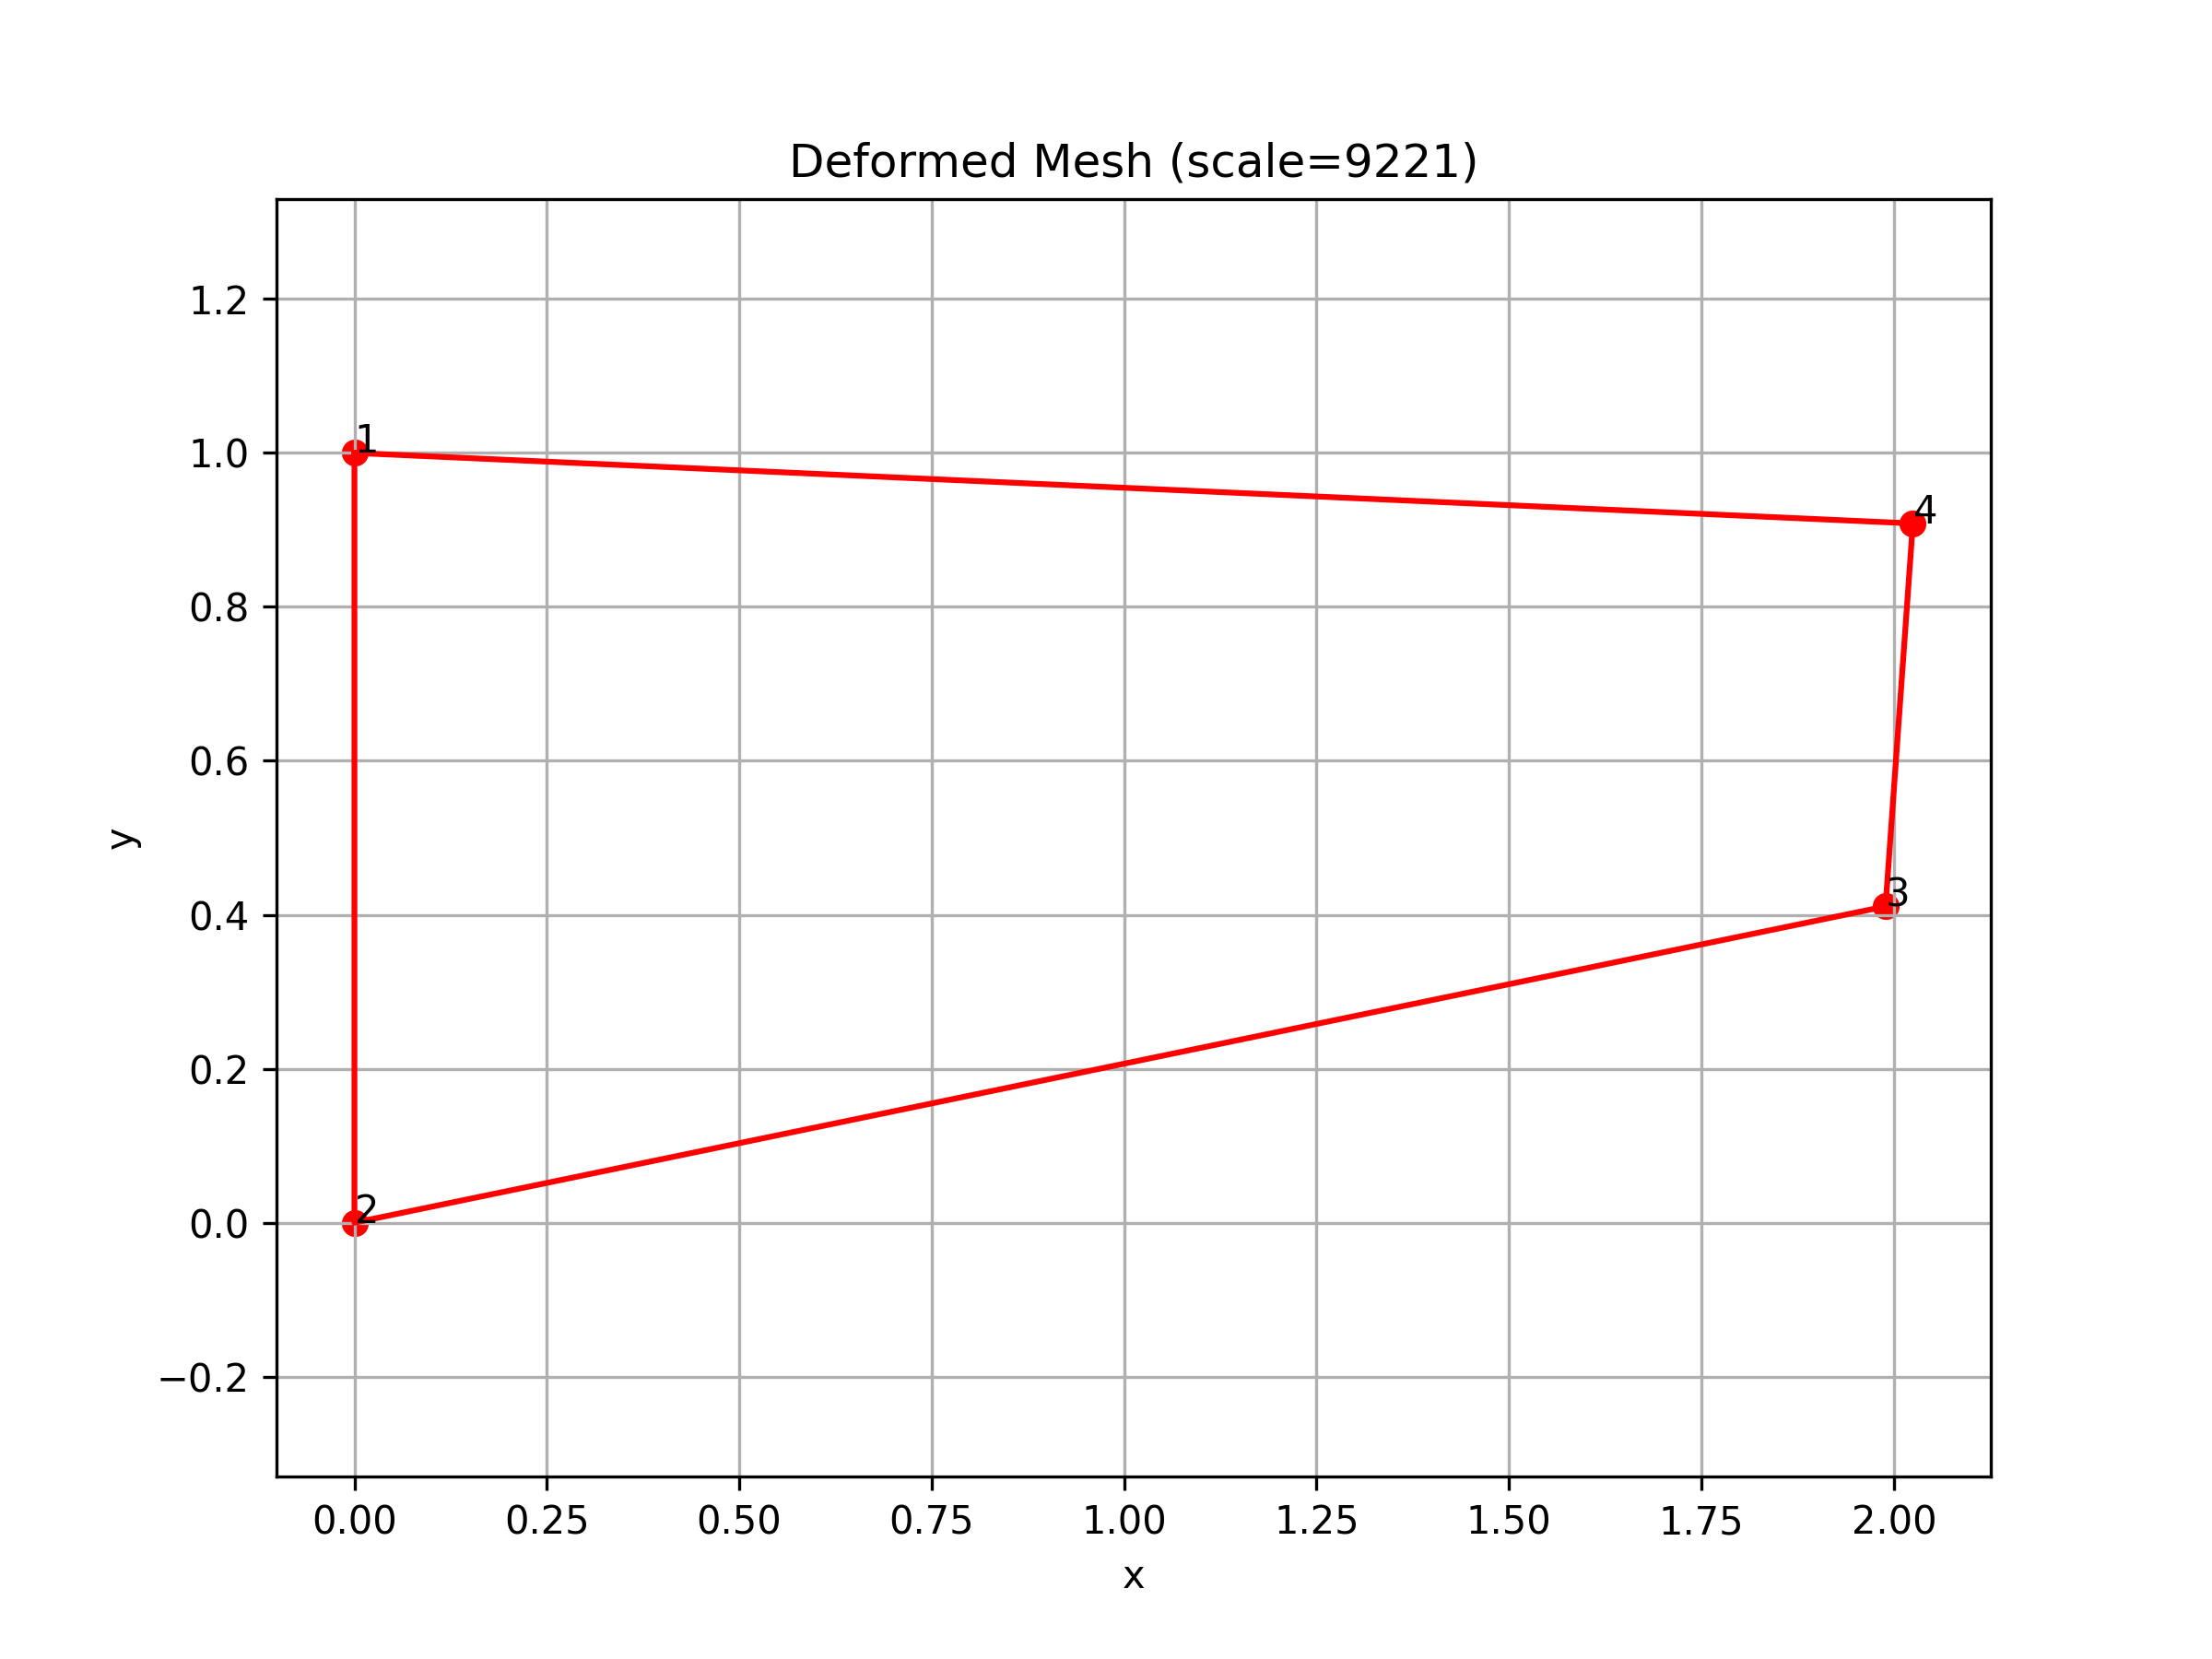
\includegraphics[width=0.8\textwidth]{data/Q4test_deformed.png}
    \caption{例题4-1——Q4单元变形图}
\end{figure}
\subsection*{4.2 分片实验}
为了验证Q4单元在不同分片下的表现,我们进行了分片实验。分片方法参考教材中的例题4-5,位移场与载荷也与例题一致。\\
其图形结构如下:
\begin{figure}[htbp]
    \centering
    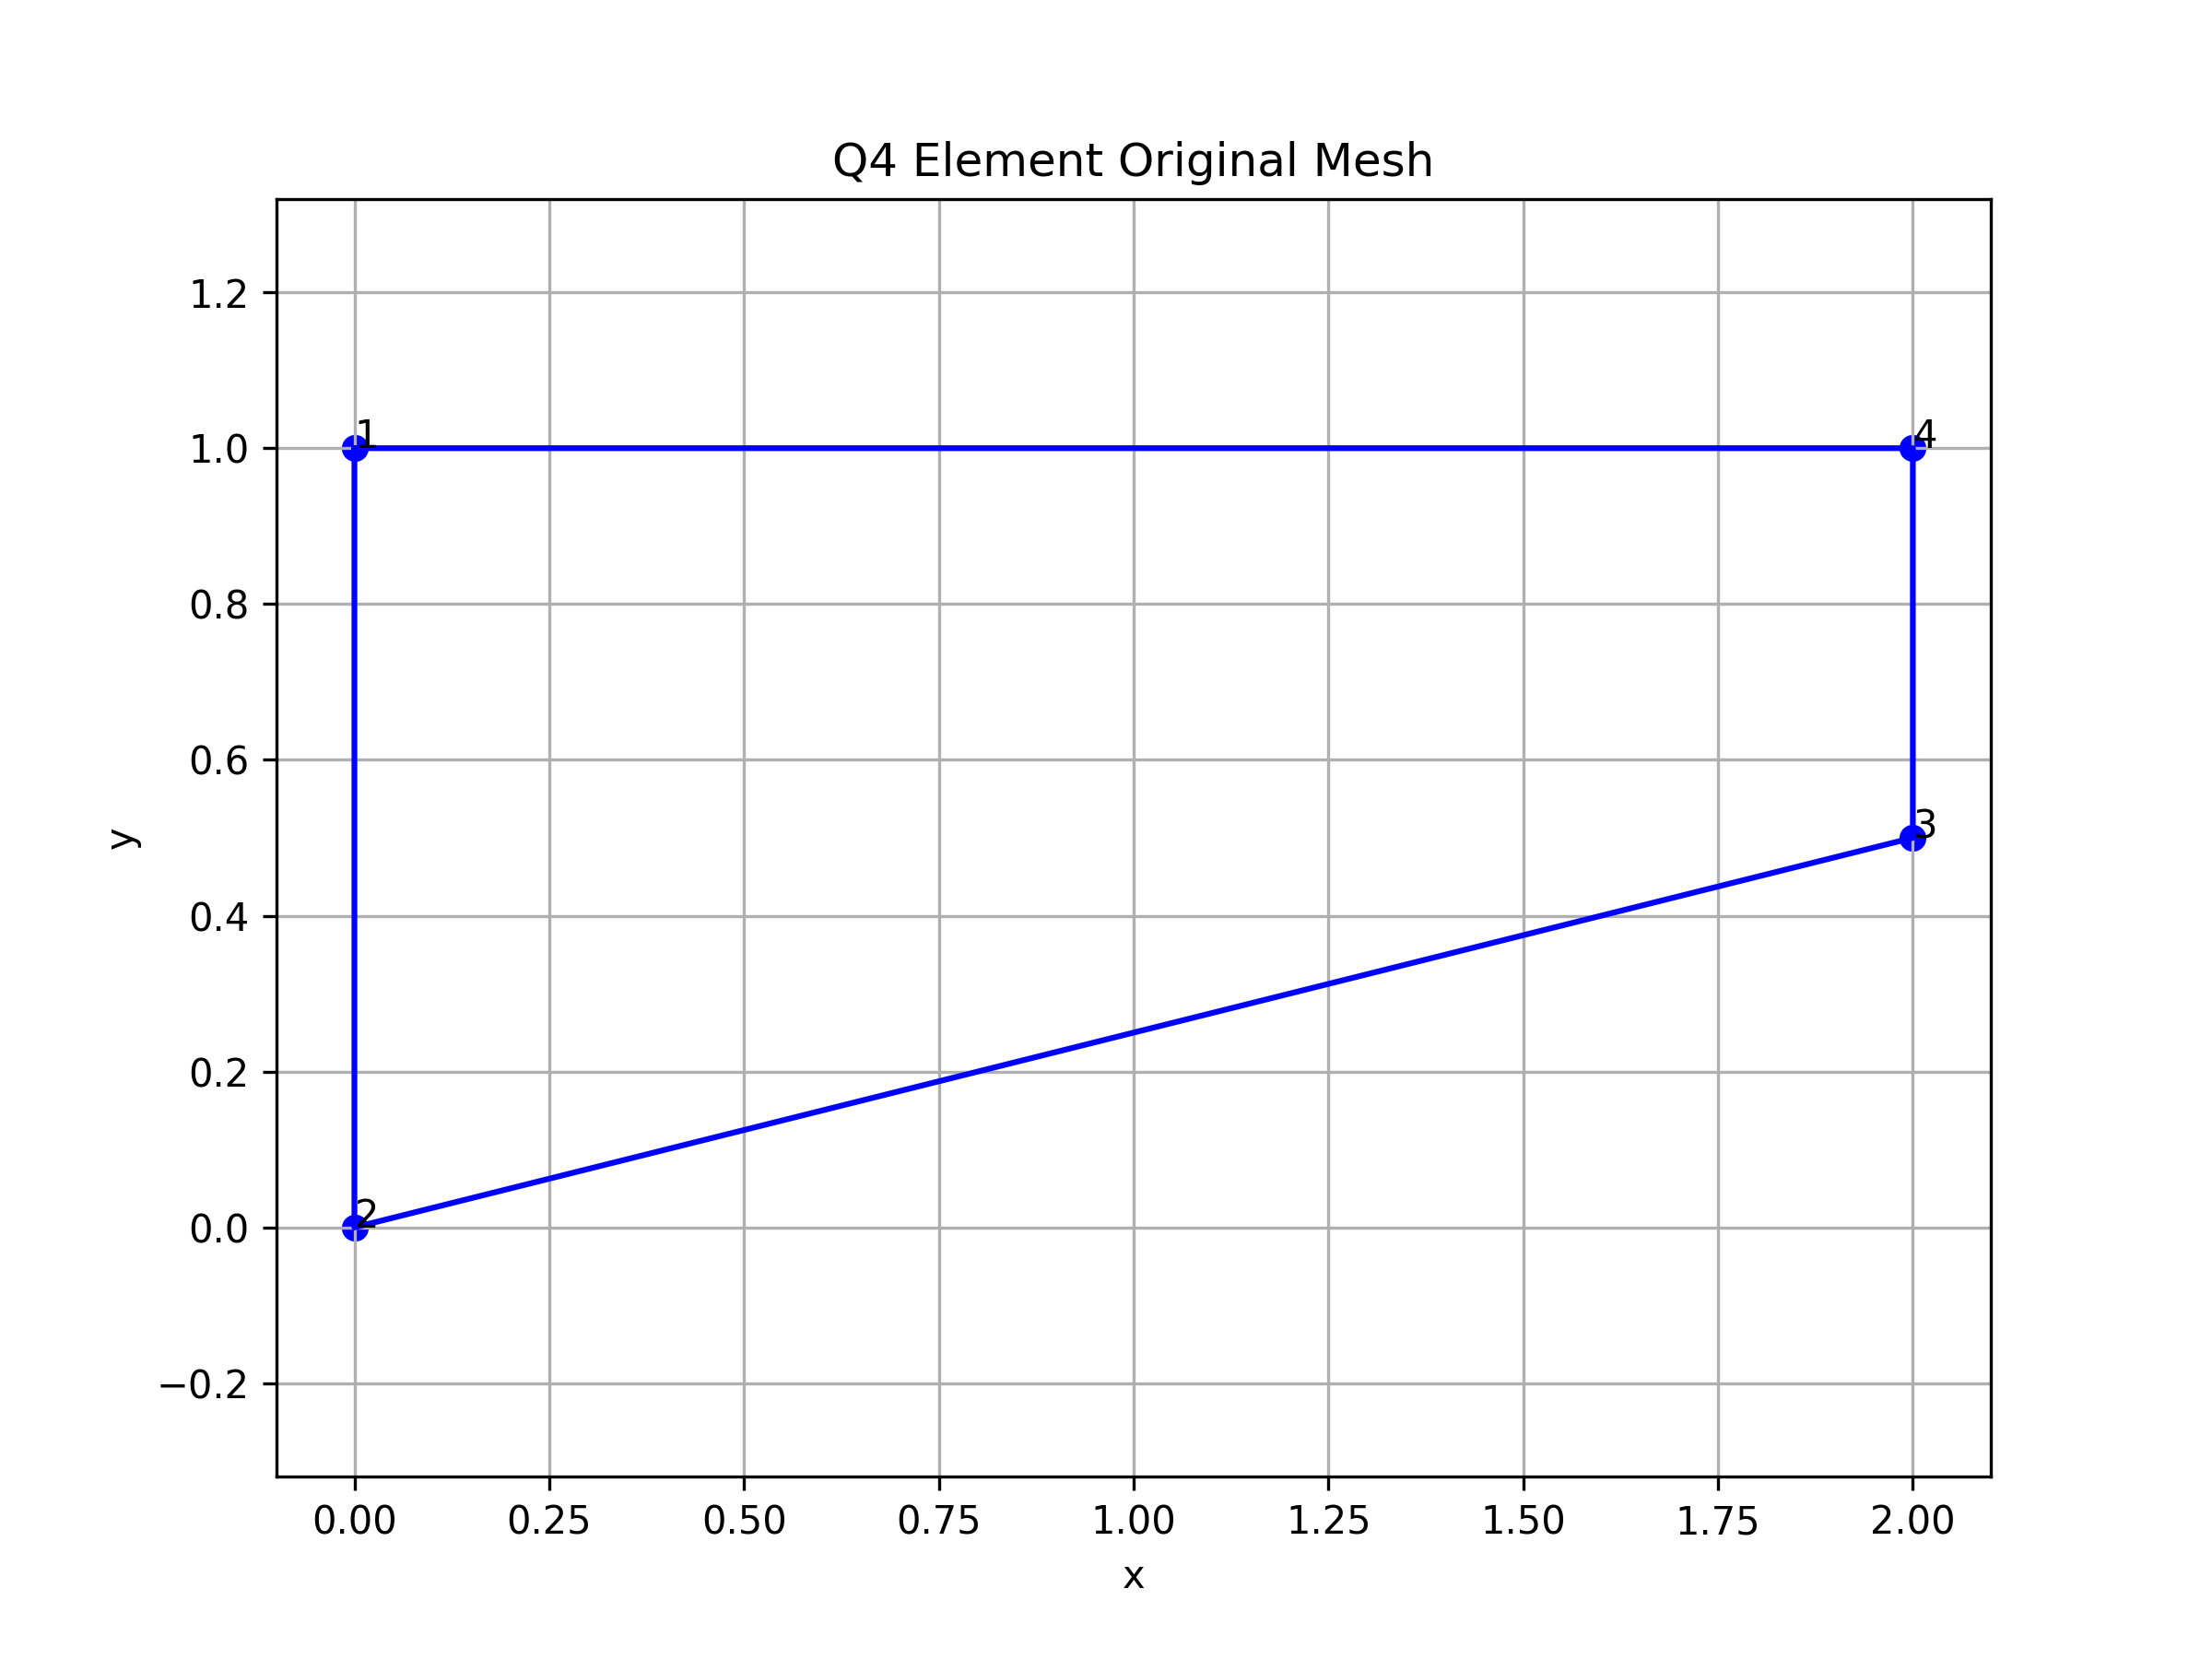
\includegraphics[width=0.8\textwidth]{data/Q4test_original.png}
    \caption{例题4-5——Q4单元分片实验图}
\end{figure}
我们采用C类分片实验,检查节点位移值是否与给定位移场相符。将输入文件保存为'patchtest.dat',运行结果如下:
\begin{lstlisting}
D I S P L A C E M E N T S

  NODE           X-DISPLACEMENT    Y-DISPLACEMENT    Z-DISPLACEMENT
    1               0.00000e+00       0.00000e+00
    2               2.50000e-02       0.00000e+00
    3               2.50000e-02      -9.00000e-03
    4               1.64799e-17      -6.00000e-03
    5               5.00000e-03      -1.50000e-03
    6               2.00000e-02      -2.25000e-03
    7               1.75000e-02      -5.25000e-03
    8               6.50000e-03      -4.80000e-03
\end{lstlisting}
与精确解的差距在可接受范围内,表明Q4单元在分片实验中的表现良好。\\
\subsection*{4.3 收敛性分析}
为了进一步验证Q4单元的收敛性,我们进行了网格划分实验。采用悬臂梁的弯曲实验进行计算,分别采用2\times 1 、4\times 2、8\times 4种网格进行计算。\\
\begin{figure}[htbp]
    \centering
    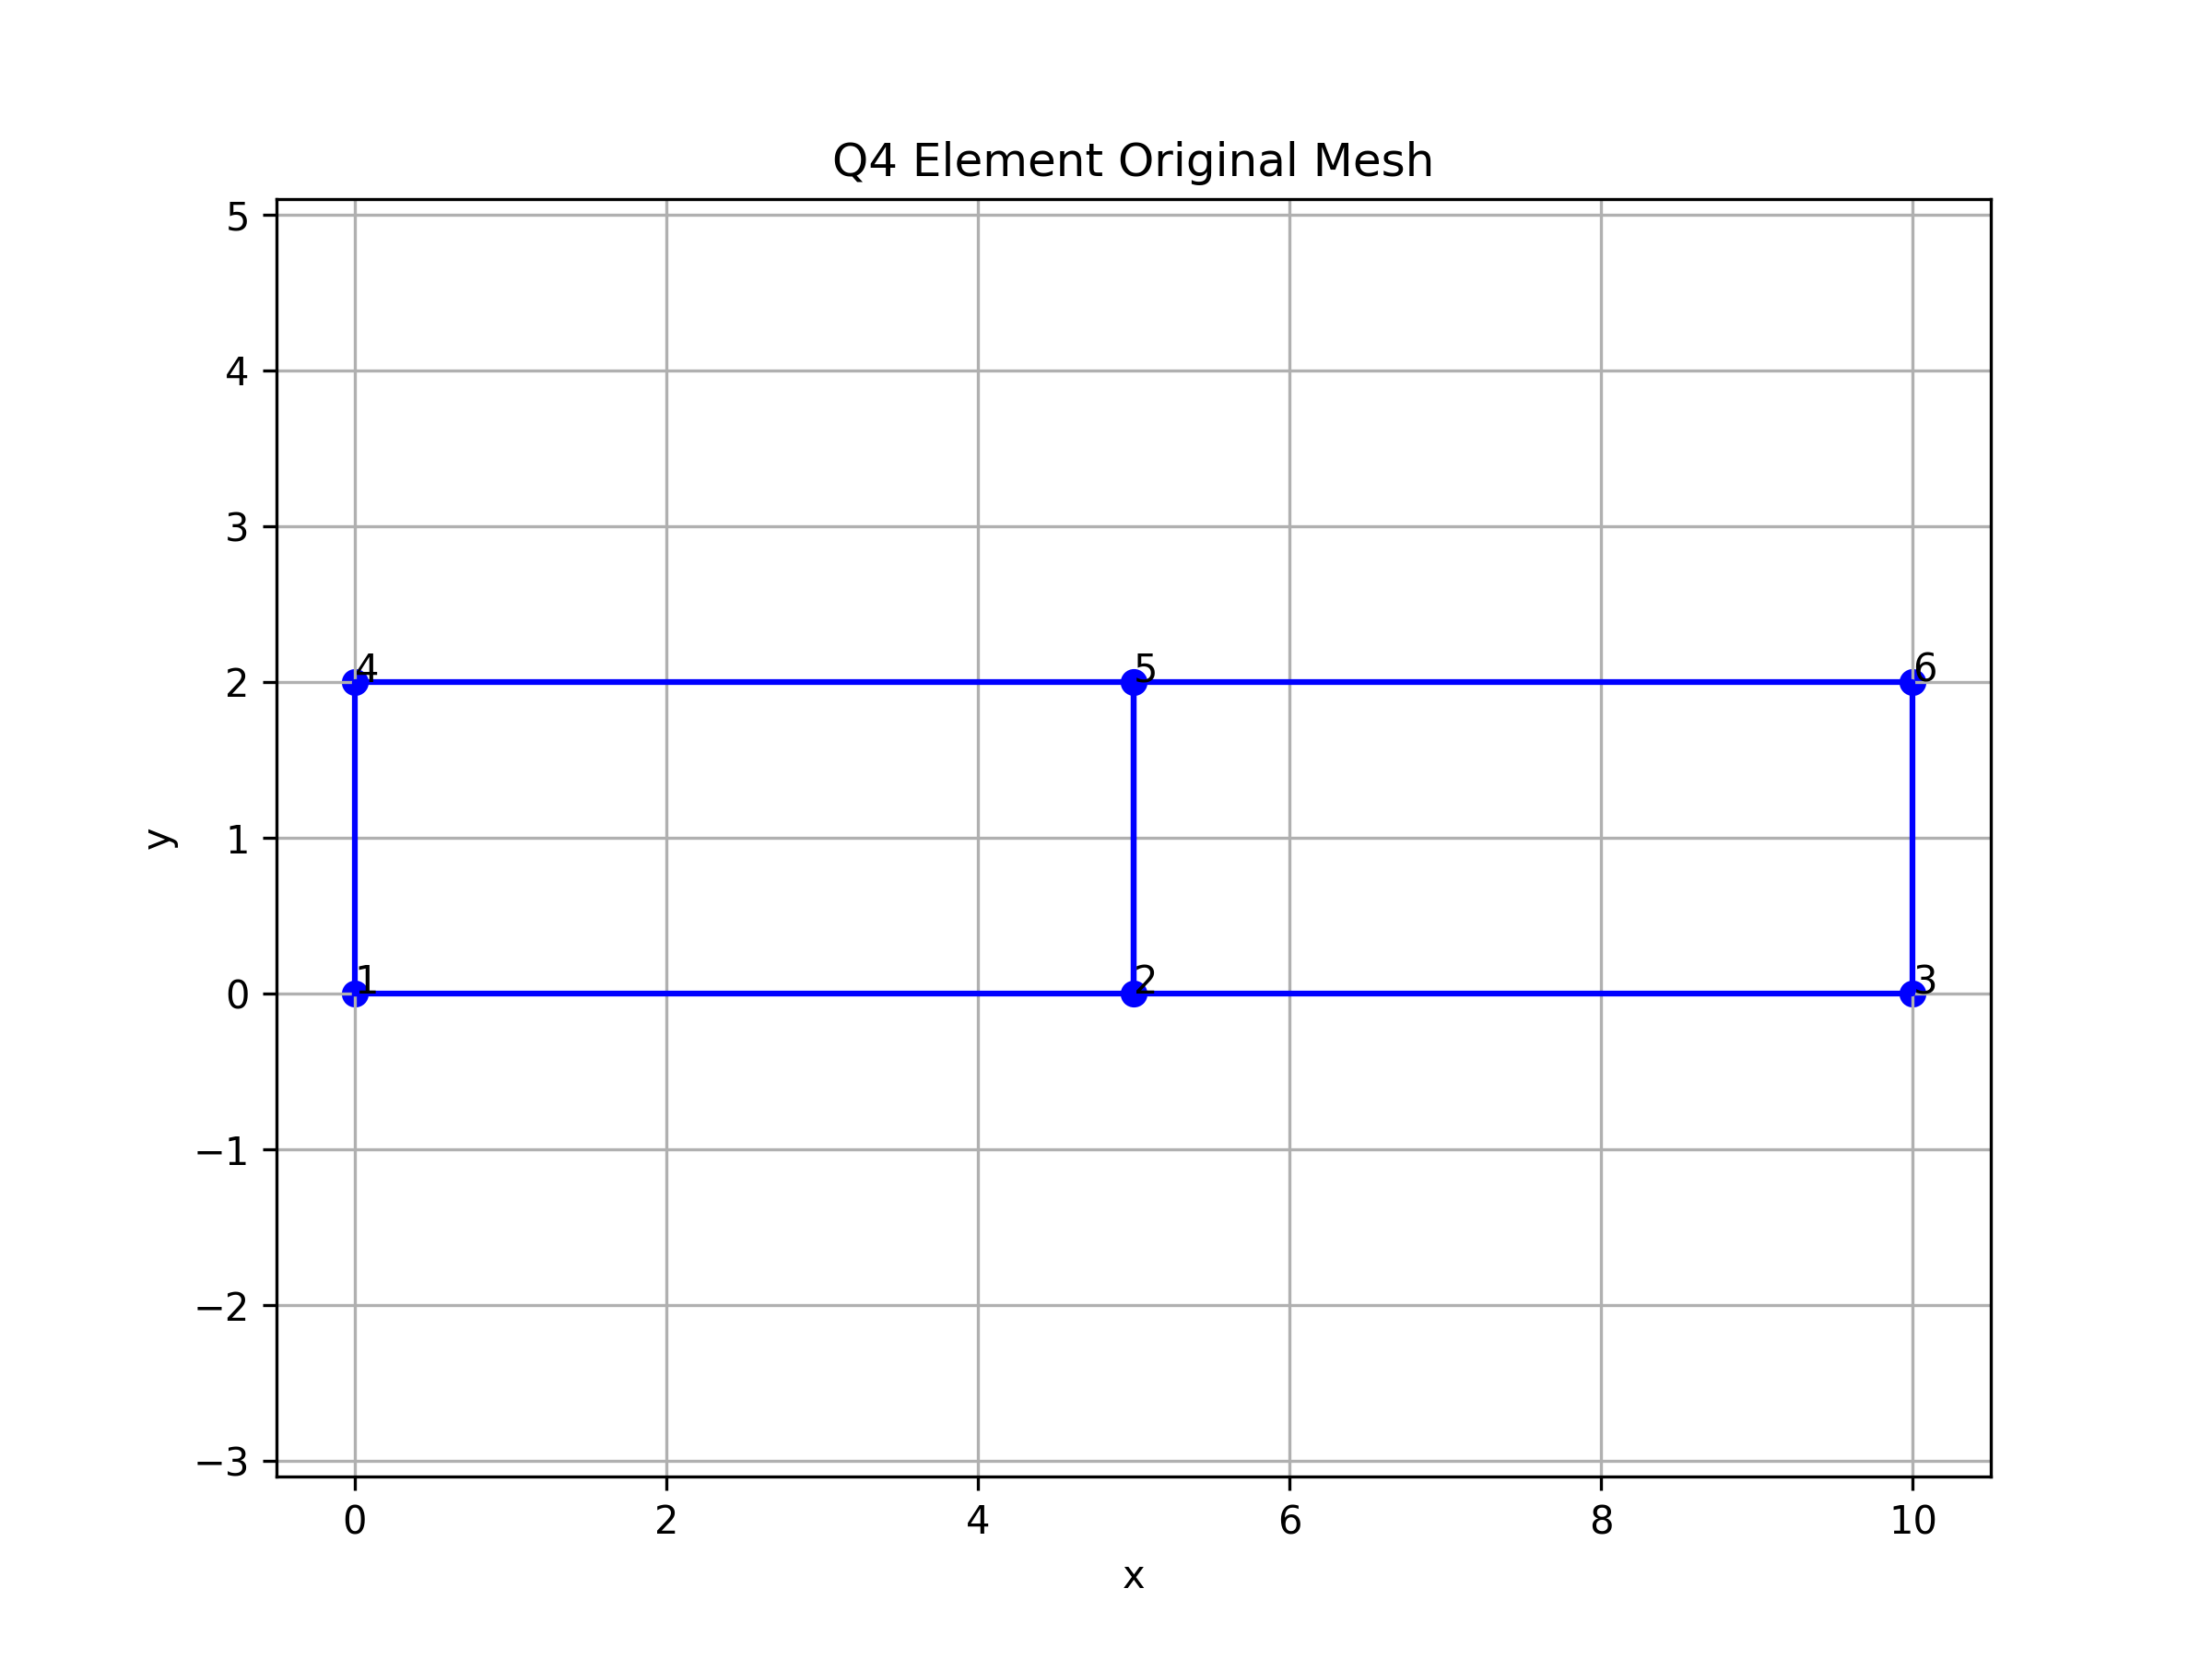
\includegraphics[width=0.8\textwidth]{data/test1_original.png}
    \caption{Q4test1}
\end{figure}
\begin{figure}[htbp]
    \centering
    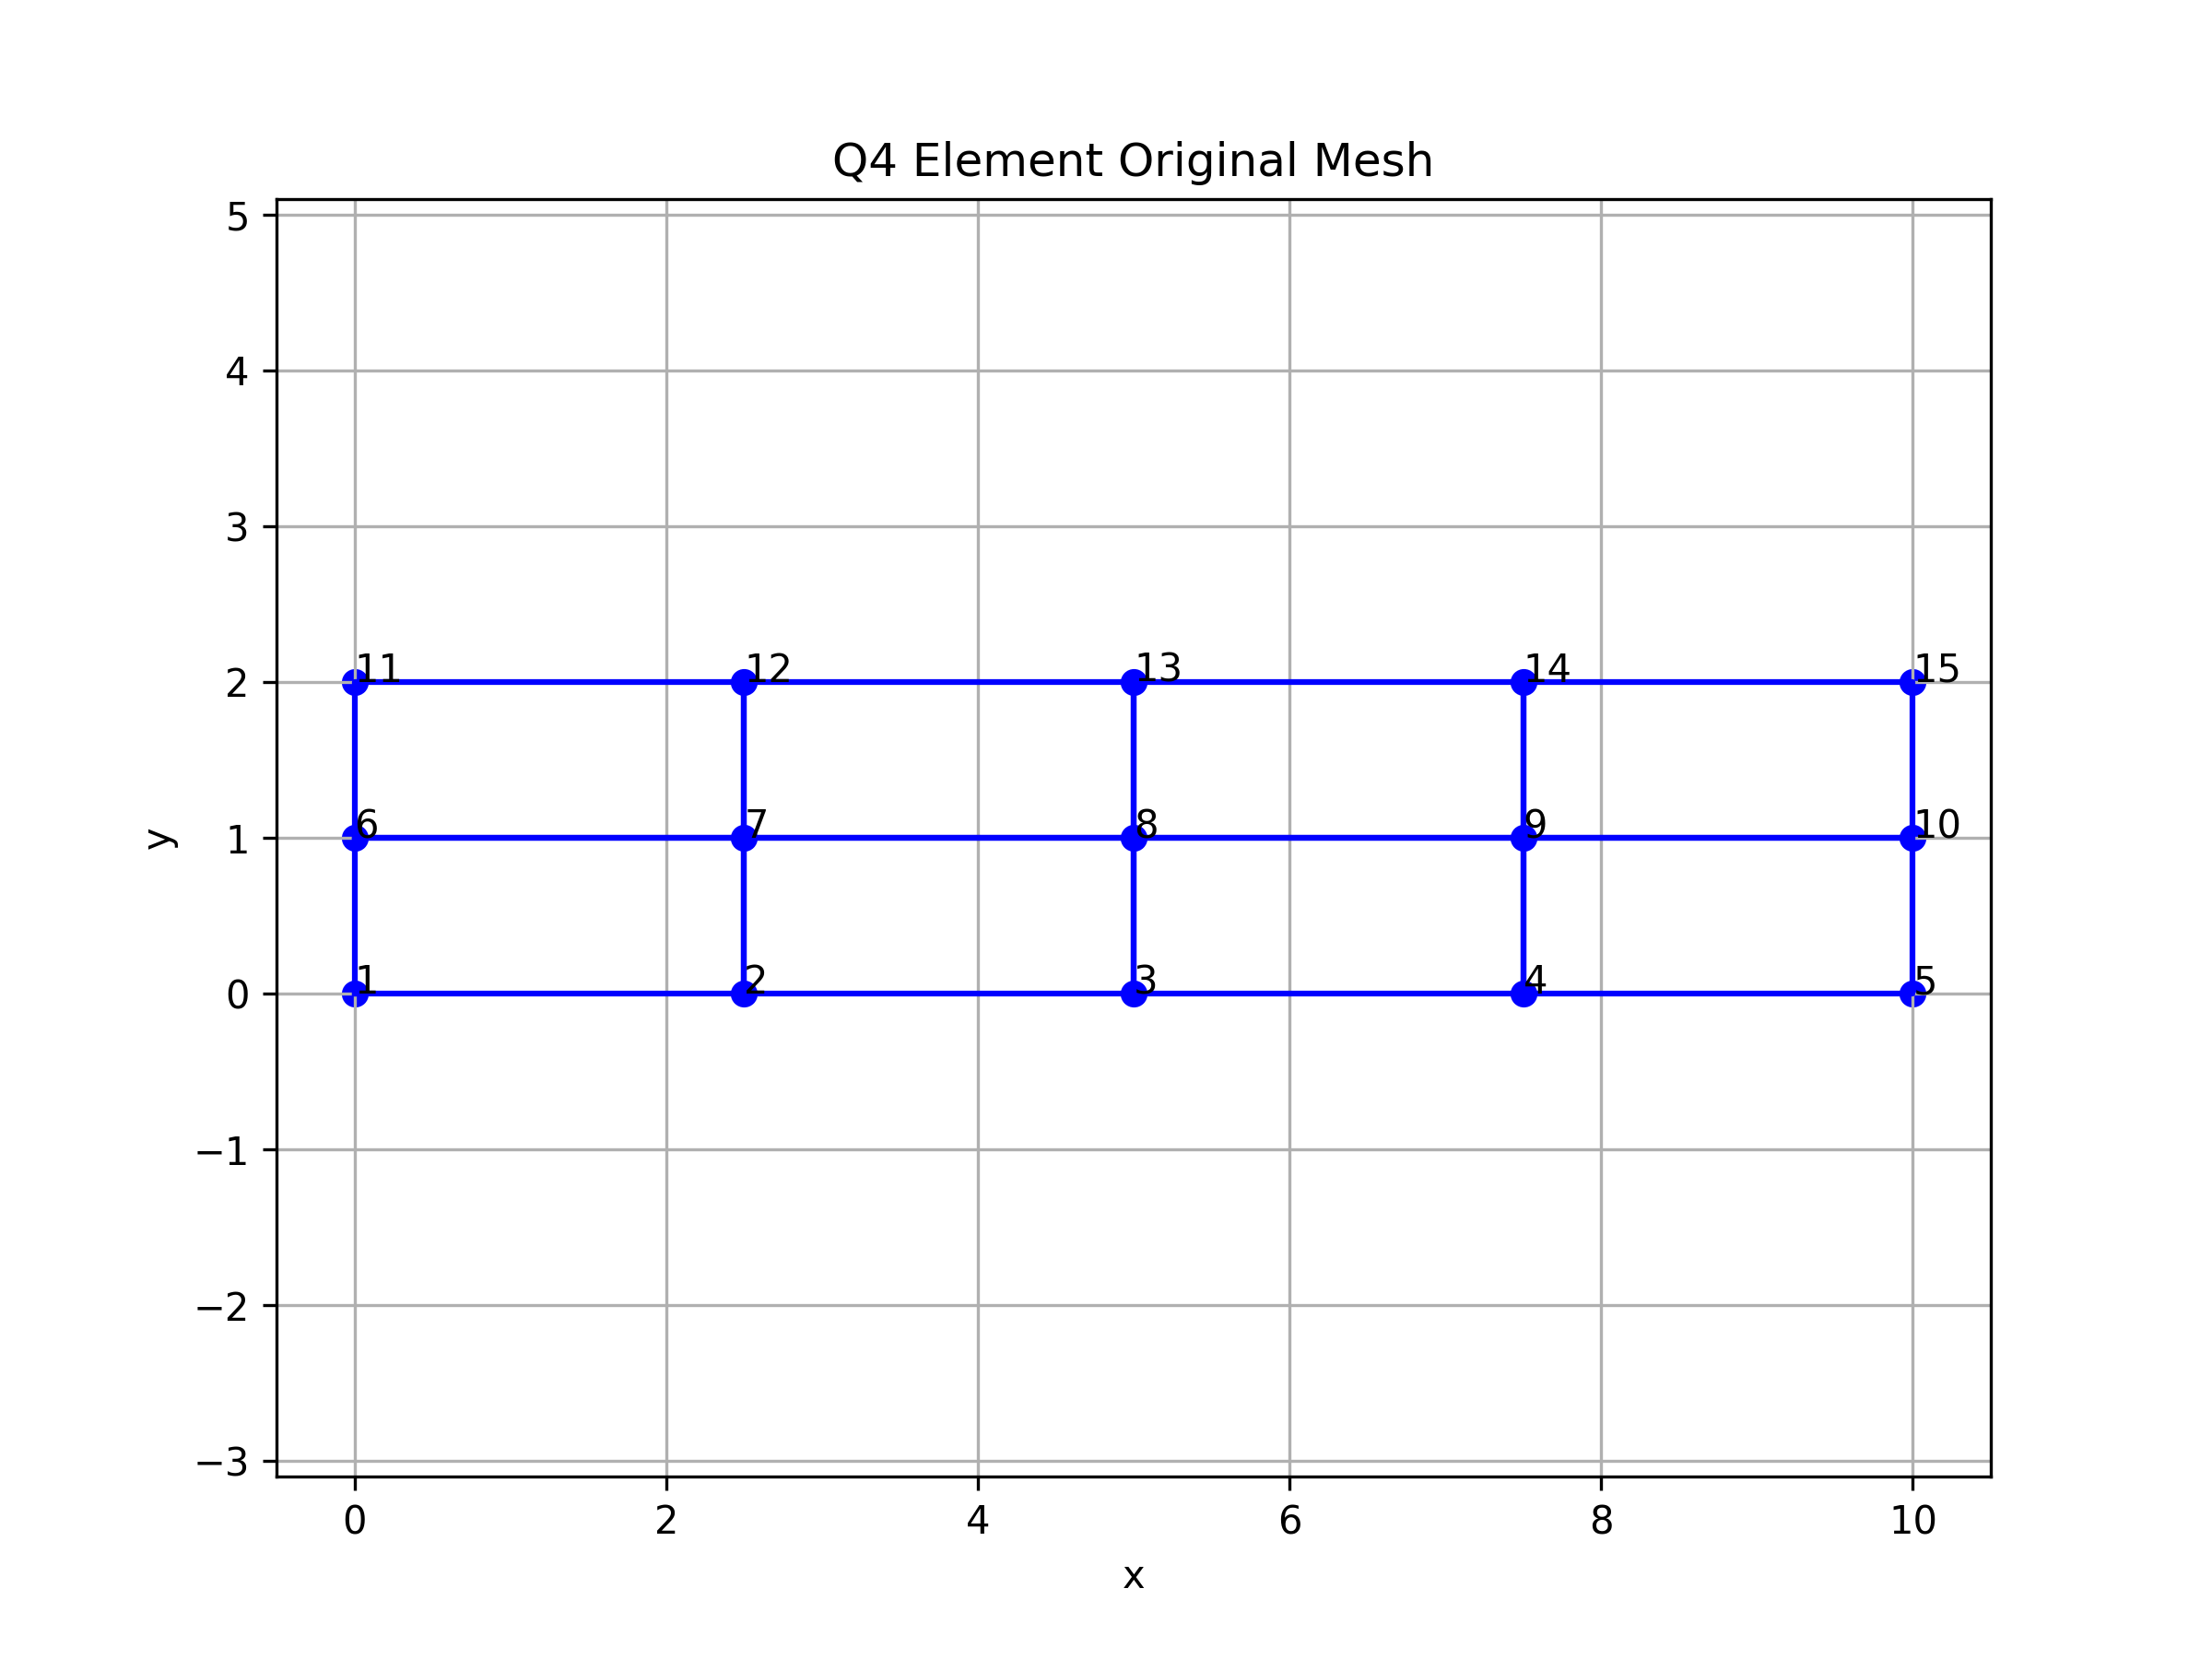
\includegraphics[width=0.8\textwidth]{data/test2_original.png}
    \caption{Q4test2}
\end{figure}
\begin{figure}[htbp]
    \centering
    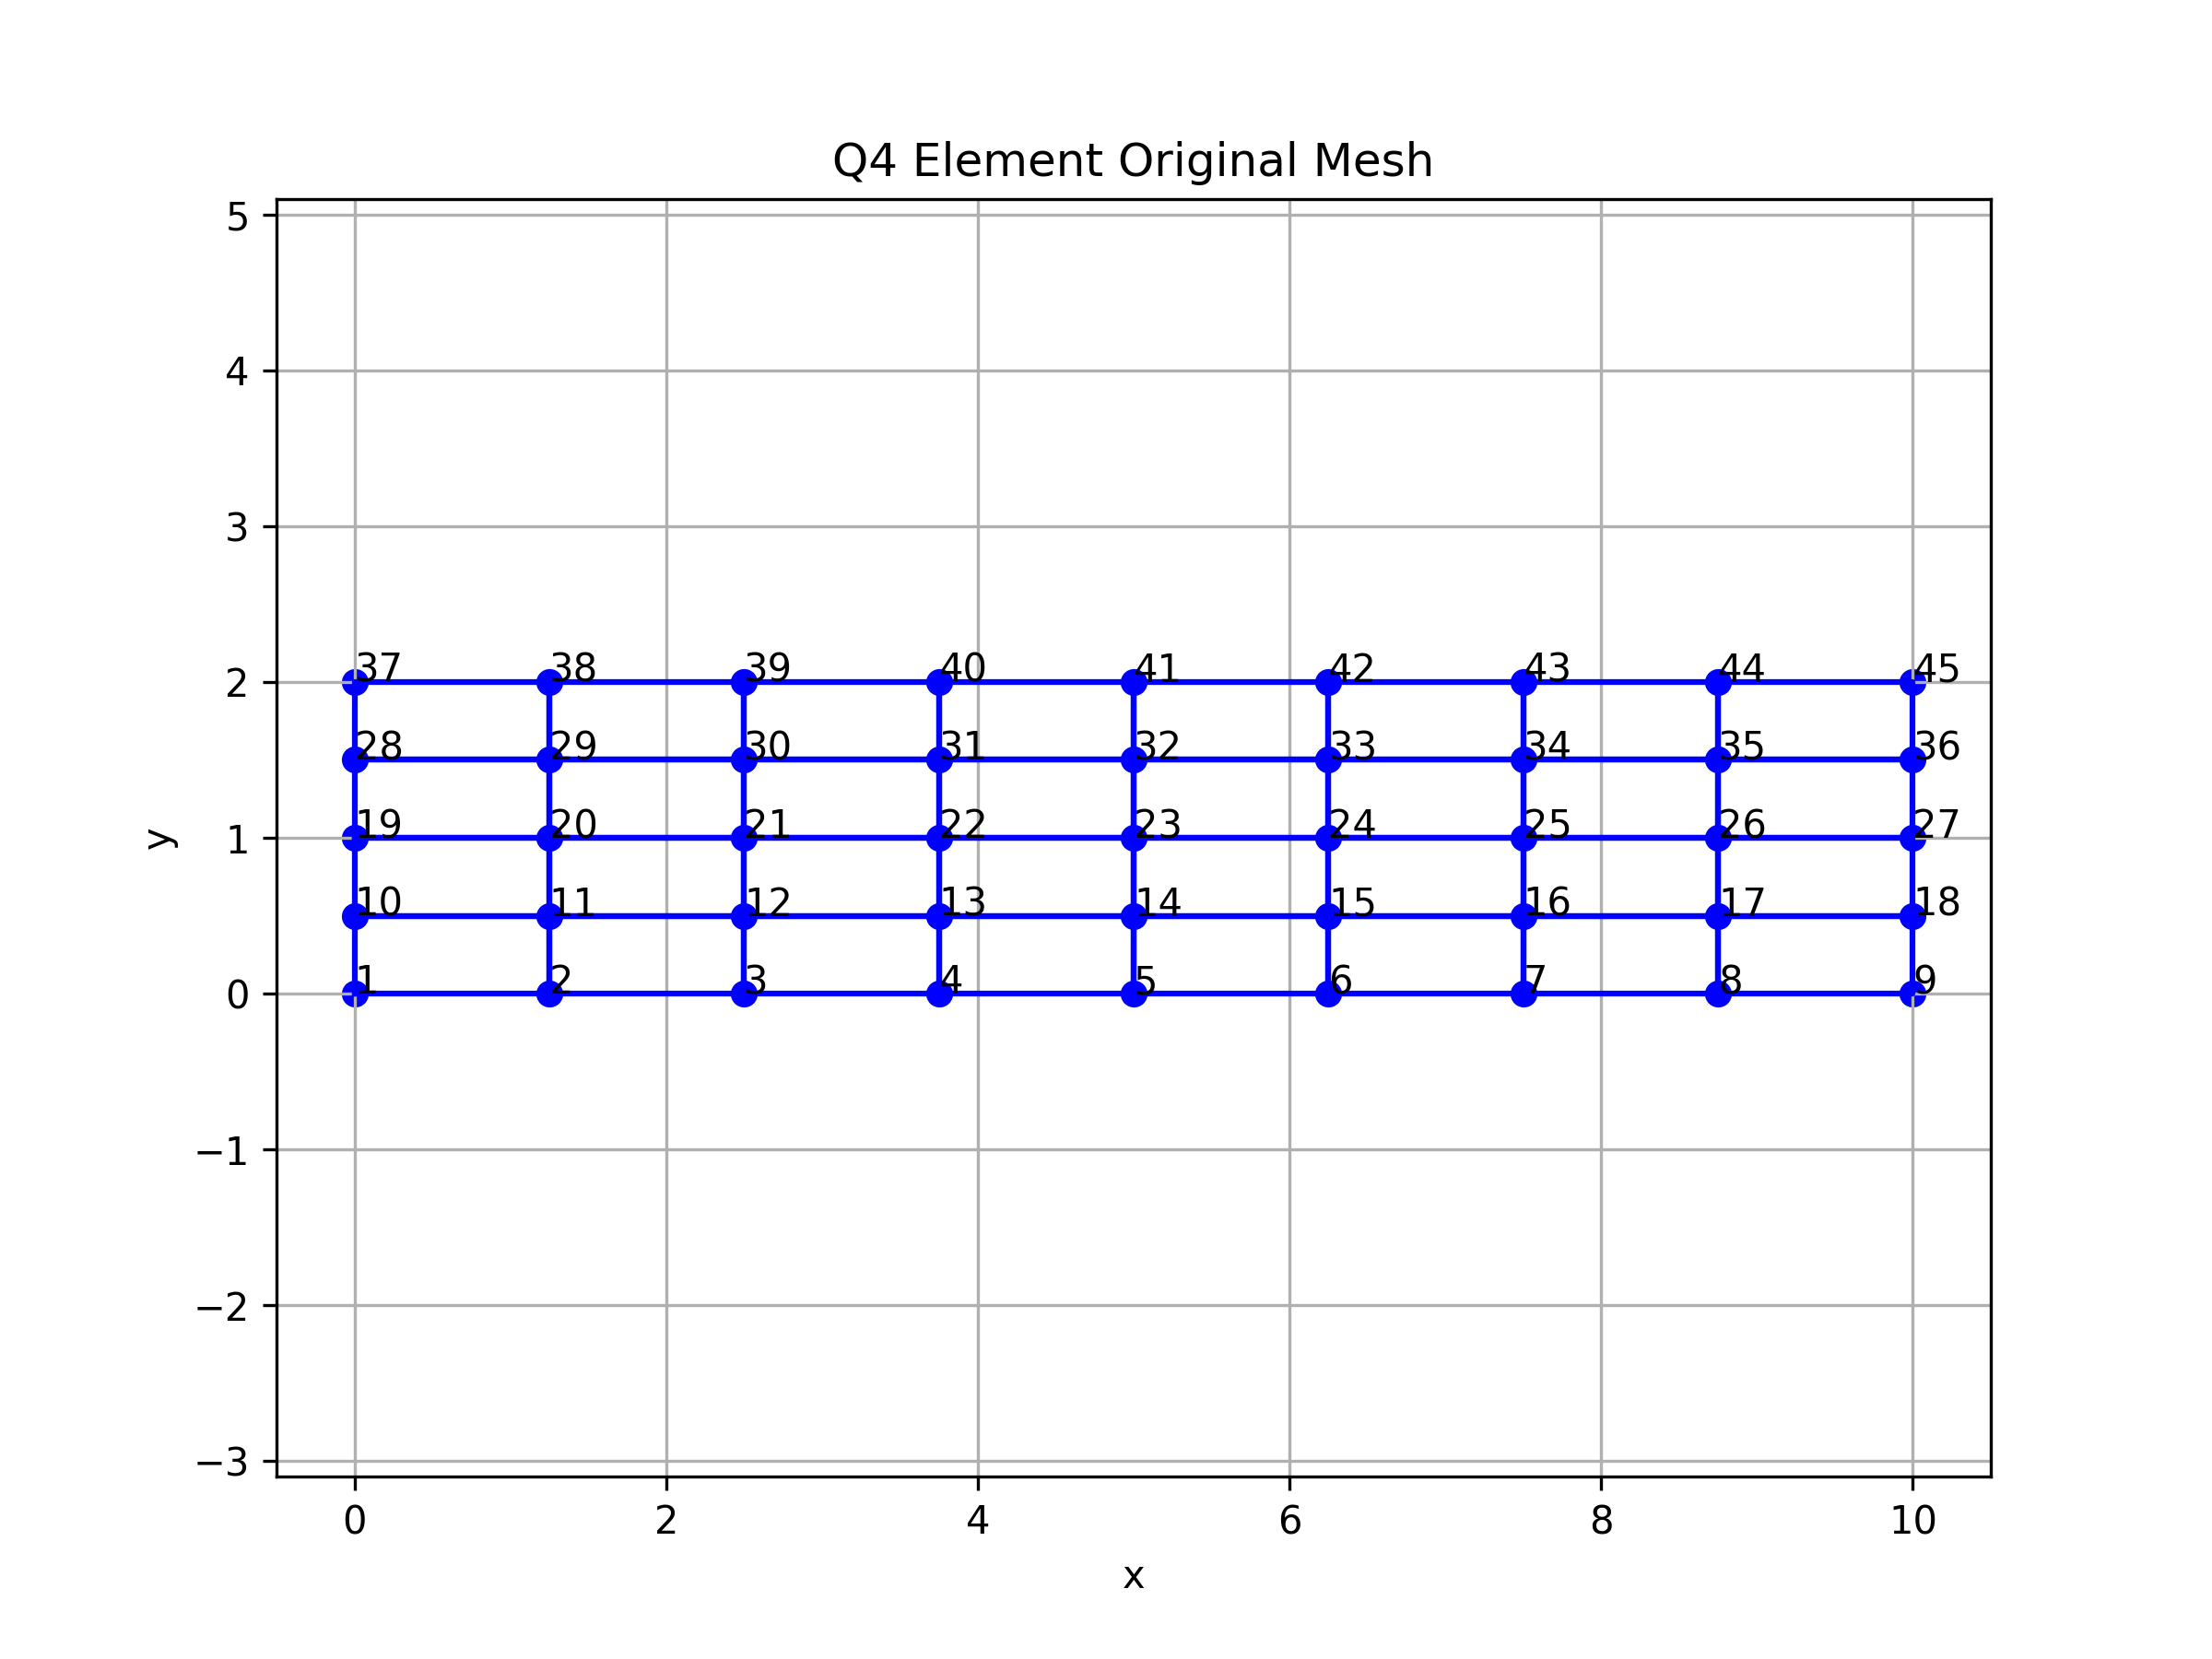
\includegraphics[width=0.8\textwidth]{data/test3_original.png}
    \caption{Q4test3}
\end{figure}
我们将输入文件保存为'test1.dat'、'test2.dat'、'test3.dat',运行后得到节点位移。随后,利用convergence.py脚本对结果进行处理,计算得到每组的L2误差。
再利用log-logplot.py脚本画出双对数图,并计算得到L2范数随单元尺寸的收敛率约为1.73,略低于理论值2,可能是因为Q4单元求解弯曲问题时会出现剪切闭锁所致。\\
\begin{figure}[htbp]
    \centering
    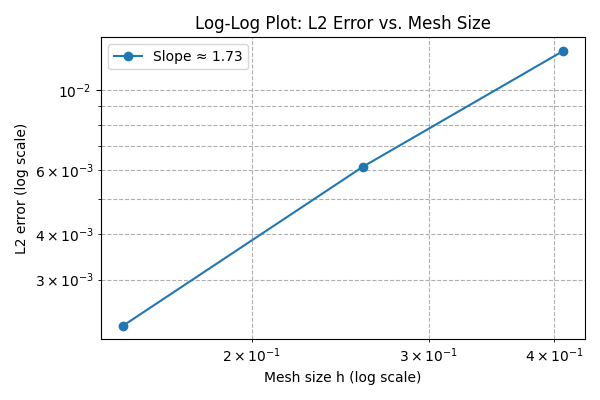
\includegraphics[width=0.8\textwidth]{data/log-log.png}
    \caption{Q4单元收敛性分析结果}
\end{figure}
\section*{五、结论}
本次作业成功实现了Q4单元的编程,并通过多个验证算例确认了其正确性。Q4单元在平面应力问题中的应用表现良好,能够有效地求解二维问题。
此外,通过分片实验和收敛性分析,我们验证了Q4单元在不同网格划分下的稳定性和收敛性。尽管存在一些剪切闭锁现象,但整体表现符合预期。\\
未来,我们可以进行更复杂的三维单元实现,或将Q4单元与其他单元结合使用,以解决更广泛的工程问题。同时,也可以探索改进Q4单元的求解方法,以提高其在弯曲问题中的表现。
\section*{六、参考文献}
\begin{enumerate}
    \item \textbf{张雄.} 有限元法基础. 高等教育出版社, 2023.
    \item \textbf{姜逸轩.} https://github.com/yixJi/STAPpp
\end{enumerate}
\end{document}